%\renewcommand{\bc}{\begin{center}}
%\renewcommand{\ec}{\end{center}}

A set of surface data is provided to serve as input for PlaSim in 3 resolutions: T21, T31 and T42. 
The file names begin with Nxxx, where xxx gives the number of latitudes of the respective resolution. 
The "mm" indicates monthly mean values (further explanation see below):\\[3.ex]
\begin{bf}T21:\end{bf}\\
\vspace{-3.8ex}
\begin{tabbing}
N032\_surf\_0173.sraxx \= abbr.xx   \= fract.xx  \= mmxx  \= Fractional vegetation \kill
\begin{bf}file name\end{bf}        \> \begin{bf}abbr.\end{bf}\>\begin{bf}unit\end{bf} \>      \> \begin{bf}variable name\end{bf}\\[0.8ex]
N032\_surf\_0129.sra \> sg   \> $m^{2}/s^{2}$ \>      \> surface geopotential orography \\
N032\_surf\_0169.sra \> tsa  \> K             \> mm   \> surface temperature accumulated \\
N032\_surf\_0172.sra \> lsm  \> fract.        \>      \> land sea mask \\
N032\_surf\_0173.sra \> z0   \> m             \>      \> roughness length \\
N032\_surf\_0174.sra \> alb  \> fract.        \> mm   \> albedo (surface background albedo) \\
N032\_surf\_0199.sra \> vegc \> fract.        \> mm   \> fractional vegetation \\
N032\_surf\_0200.sra \> lai  \>               \> mm   \> leaf area index \\
N032\_surf\_0210.sra \> sic  \> \%            \> mm   \> sea ice cover \\
N032\_surf\_0212.sra \> vegf \> fract.        \>      \> forest ratio \\
N032\_surf\_0229.sra \> mrfc \> m             \>      \> maximum soil water holding (field) capacity \\
N032\_surf\_0232.sra \> glac \> fract.        \>      \> glacier fraction  \\
N032\_surf\_1730.sra \> z0t  \> m             \>      \> roughness length due to topography \\
N032\_surf\_1731.sra \> z0v  \> m             \>      \> roughness length due to vegetation and land use\\
N032\_surf\_1740.sra \> albs \> fract.        \>      \> bare soil albedo \\
N032\_surf\_1741.sra \> albv \> fract.        \>      \> albedo due to vegetation \\
\end{tabbing}

\vspace{-1.6ex}
\noindent \begin{bf}T31:\end{bf}\\
file names begin with: N048 \\

\noindent \begin{bf}T42:\end{bf}\\
file names begin with: N064 \\
\vspace{3.ex}

The format of the files is "service ascii". They are opened as {\small FORMATTED} files and can be read as:

\begin{tabbing}
xxxxxxx \= integer \=::x\=field(nlon,nlat) \kill
        \> integer \>::\>ih (8)\\
        \> real    \>::\>field (nlon,nlat)\\[0.8ex]
xxxxxxx \= open(filenr,file='N....sra',form='{\small FORMATTED}') \kill
        \> open(filenr,file='N....sra',form='{\small FORMATTED}') \\
xxxxxxx \= read(filenr,)x \= field \kill
        \> read(filenr,*)    \> ih \\
        \> read(filenr,*)    \> field \\
\end{tabbing}

As the files contain formatted data, any text editor could be used to view or change the data as well.\\
The data of tsa (code 169), alb (code 174), vegc (code 199), lai (code 200) and sic (code 210) are stored as 
14 monthly mean fields (indicated by the "mm" in the table above): 
Jan to Dec are months 1 to 12 with Dec duplicated as month 0 and Jan duplicated as month 13.\\
All other files contain one yearly mean field.\\

\section{Source}
 The data are obtained from four different sources:
\subsection{codes: 174, 199, 200, 212, 229, 232, 1731}
These data are obtained from the LSP dataset of the U.S. Geological Survey, 
which is based on a 1km global distribution of major ecosystem types.\\
They are part of a dataset provided by Stefan Hagemann, MPI Hamburg in T21, T31 and T42 resolution. 
A detailed description can be found in two MPI scientific reports\\ \cite{hagemann1999} and \cite{hagemann2002}.\\
The values refer to the land part of the grid box.

\subsection{codes: 173, 1730 \hspace{1.ex} and 129, 172}
The data of the "roughness length due to topography" and therefore the total roughness length as well are not
included in the above mentioned dataset. $z0_t$ (code 1730) was calculated by MPI Hamburg (and provided by Uwe Schulzweida)
as ECHAM input from the GTOPO30 dataset of the U.S. Geological Survey (\url{http://eros.usgs.gov}), which is regularly spaced
 at 30-arc seconds (app. 1km). The method is described in \cite{tibaldi1981}.\\
$z0$ (code 173) is calculated using:
\begin{equation}
{z0} = \sqrt{z0_t^{2} + z0_v^{2}}
\label{r0_eq}
\end{equation}
according to \cite{hagemann1999}.\\
The surface geopotential ($= g *$ Topography [m]) and the land sea mask are also derived from the GTOPO30 dataset. 
An area-true interpolation to the Gaussian grid is used.

\subsection{codes: 1740, 1741, 174}
The data were provided by Diana Rechid, MPI Hamburg, as global fields with $0.5^\circ$ resolution. 
A description on the method is available at \cite{rechid2009} and \cite{rechid2008}. The values 
refer to the land part of the grid box. They base on MODIS satellite data of the years 2001-2004 
and do not represent land use change.\\
The soil albedo and the vegetation albedo are given as one yearly field. The albedo (code 174) is
calculated from those two parts and from the monthly mean values of lai (code 200) to get a 
yearly cycle.

\subsection{codes: 169, 210}
The sea ice cover and the surface temperature are calculated from the AMIP-II boundary condition dataset 
(\url{http://www-pcmdi.llnl.gov/projects/amip}) as multi year monthly mean values over the whole time period (1870-2006).
The surface temperature is given in AMIP-II as sea surface temperature which is also defined for 
land points in order to enable land sea mask modifications without changing the SST field.
The data were provided by Karl Taylor, PCMDI, on Gaussian grid in resolutions T21, T31 and T42.

\section{Modification}
The fields described above (except codes 129, 172, 169 and 210) are composed of useful values on land points
 and missing values or 
dummy values on sea points. The land sea mask of the data does not match the (currently) used 
land sea mask of PlaSim exactly, and probably the PlaSim land sea mask will be changed slightly for 
some simulations. To avoid the problem that some land points might not get proper values of surface data,
we decided to extend the land point values to the sea points.\\
This is done as follows:

\noindent All gridpoints with: \\
\vspace{-4.ex}
\begin{tabbing}
xxxxxxxx \= {\it value} .lt. 0.0001 {\small .AND.} lsm .le. 0.005 \kill
         \> {\it value} .lt. 0.0001 {\small .AND.} lsm .le. 0.005 \\
\end{tabbing}
\vspace{-4.ex}
are considered as changeable sea points.\\

\noindent The {\it value} is replaced by the {\it value} of the left and/or right neighboring point.
Therefore the neighboring point has to meet the requirements: \\
\vspace{-4.ex}
\begin{tabbing}
xxxxxxxx \= {\it value} .ge. 0.0001 {\small .OR.}  lsm .gt. 0.005 \kill
         \> {\it value} .ge. 0.0001 {\small .OR.}  lsm .gt. 0.005 \\
\end{tabbing}
\vspace{-4.ex}
If only one neighboring point fulfills this condition, the value is taken,\\     
if both neighboring points fulfill this condition, the average of their values is taken, \\    
if no neighboring point fulfills this condition, the value stays unchanged until the next iteration.\\     

ATTENTION: For this reason the resulting fields have to be modified by the used 
land sea mask to mask out the values on sea points!!!\\



\noindent {\bf Additions / Exceptions:}\\
\vspace{-4.ex}
\begin{tabbing}
1. \= lower limit for z0 (code 173) and z0t (code 1730) is set to 0.0001m\kill
1. \> lower limit for z0 (code 173) and z0t (code 1730) is set to 0.0001m\\
2. \> lower limit for "Maximum soil water holding (field) capacity" (code 229) is set to 0.001m, \\
   \> units are set to [m] (from [mm]).\\
3. \> threshold value (for gridpoints to change, see above) for z0 (code 173) and \\ 
   \> albedo (codes 1740,1741,174) is set to 0.5 instead of 0.005\\
4. \> only for T31-fields: for vegc (code 199) and lai (code 200), the threshold value \\
   \> for lsm is set to 0.5 instead of 0.005\\
\end{tabbing}

\section{Examples}
As an example the fields in T21 resolution are shown. For sg, tsa, lsm and sic the whole fields are plotted,
for all other fields only gridpoints with lsm $> 0.005$, which are considered as land points.\\
\noindent For alb, vegc, lai, tsa and sic the fields of January and July are shown.
\vspace{2.ex}

\begin{figure}[ht] \bc
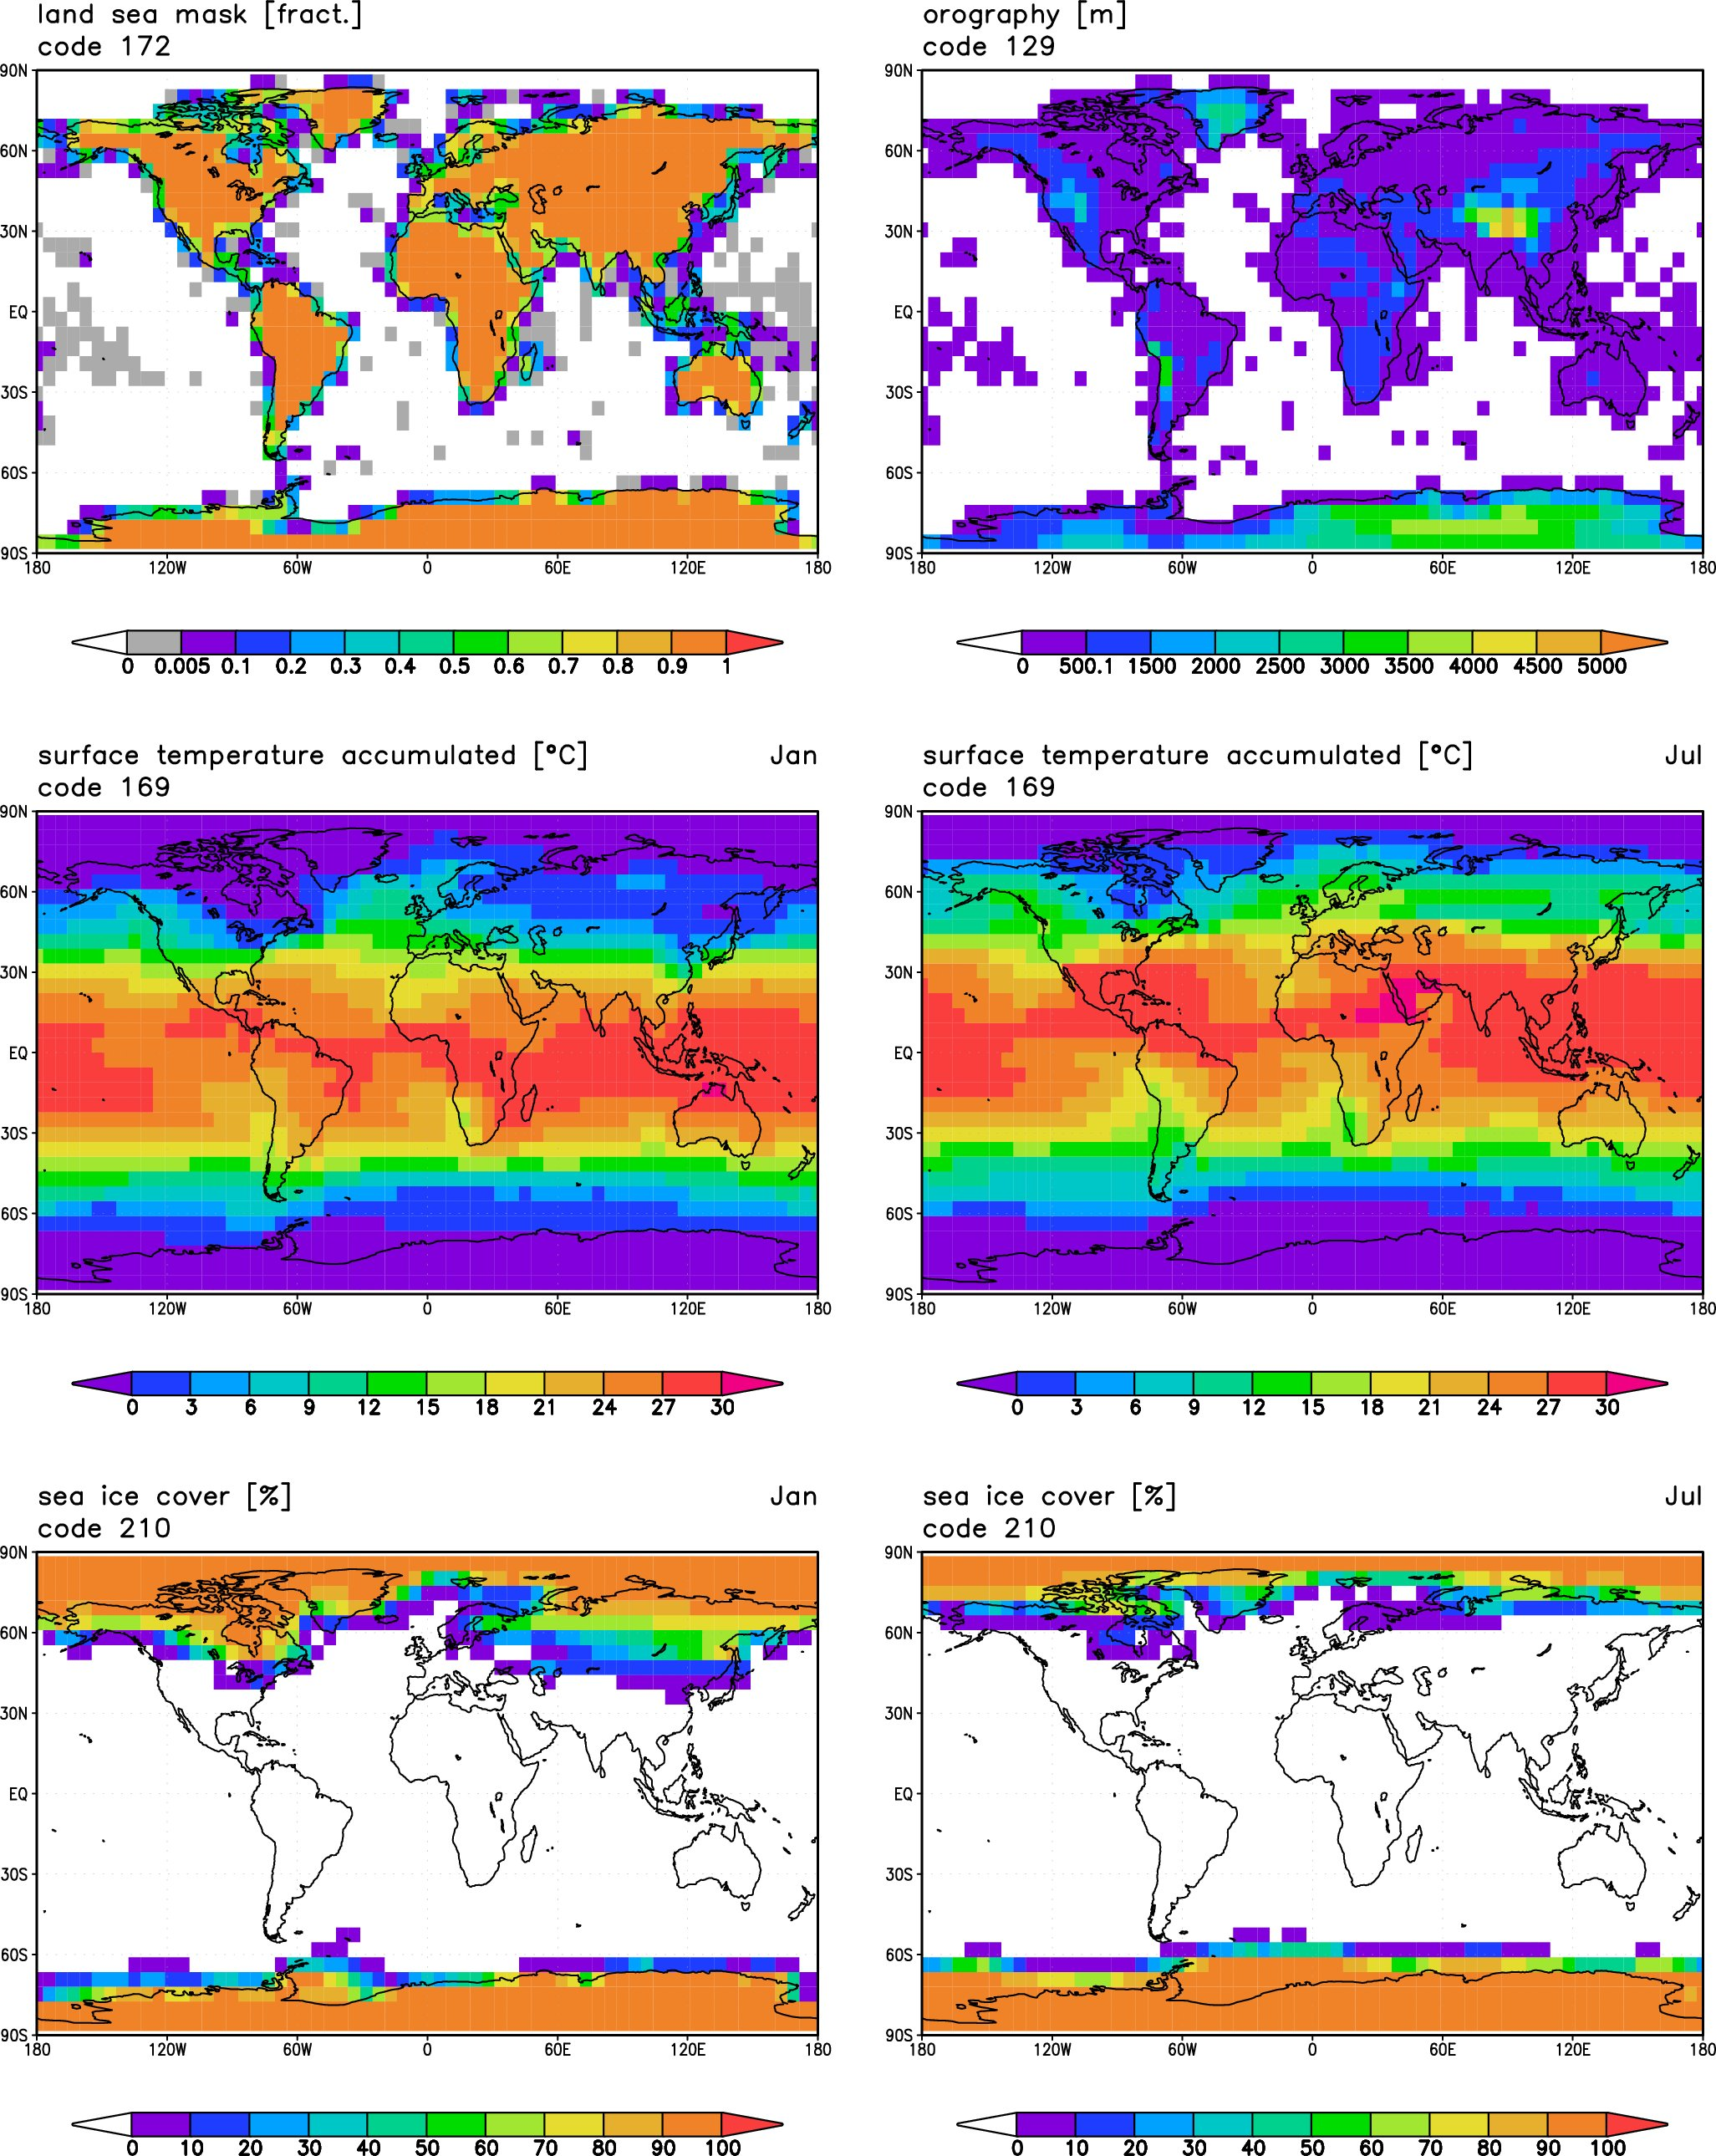
\includegraphics{silke/surface_fields_for_UG_Edi}
\ec \end{figure}

\begin{figure} [ht] \bc
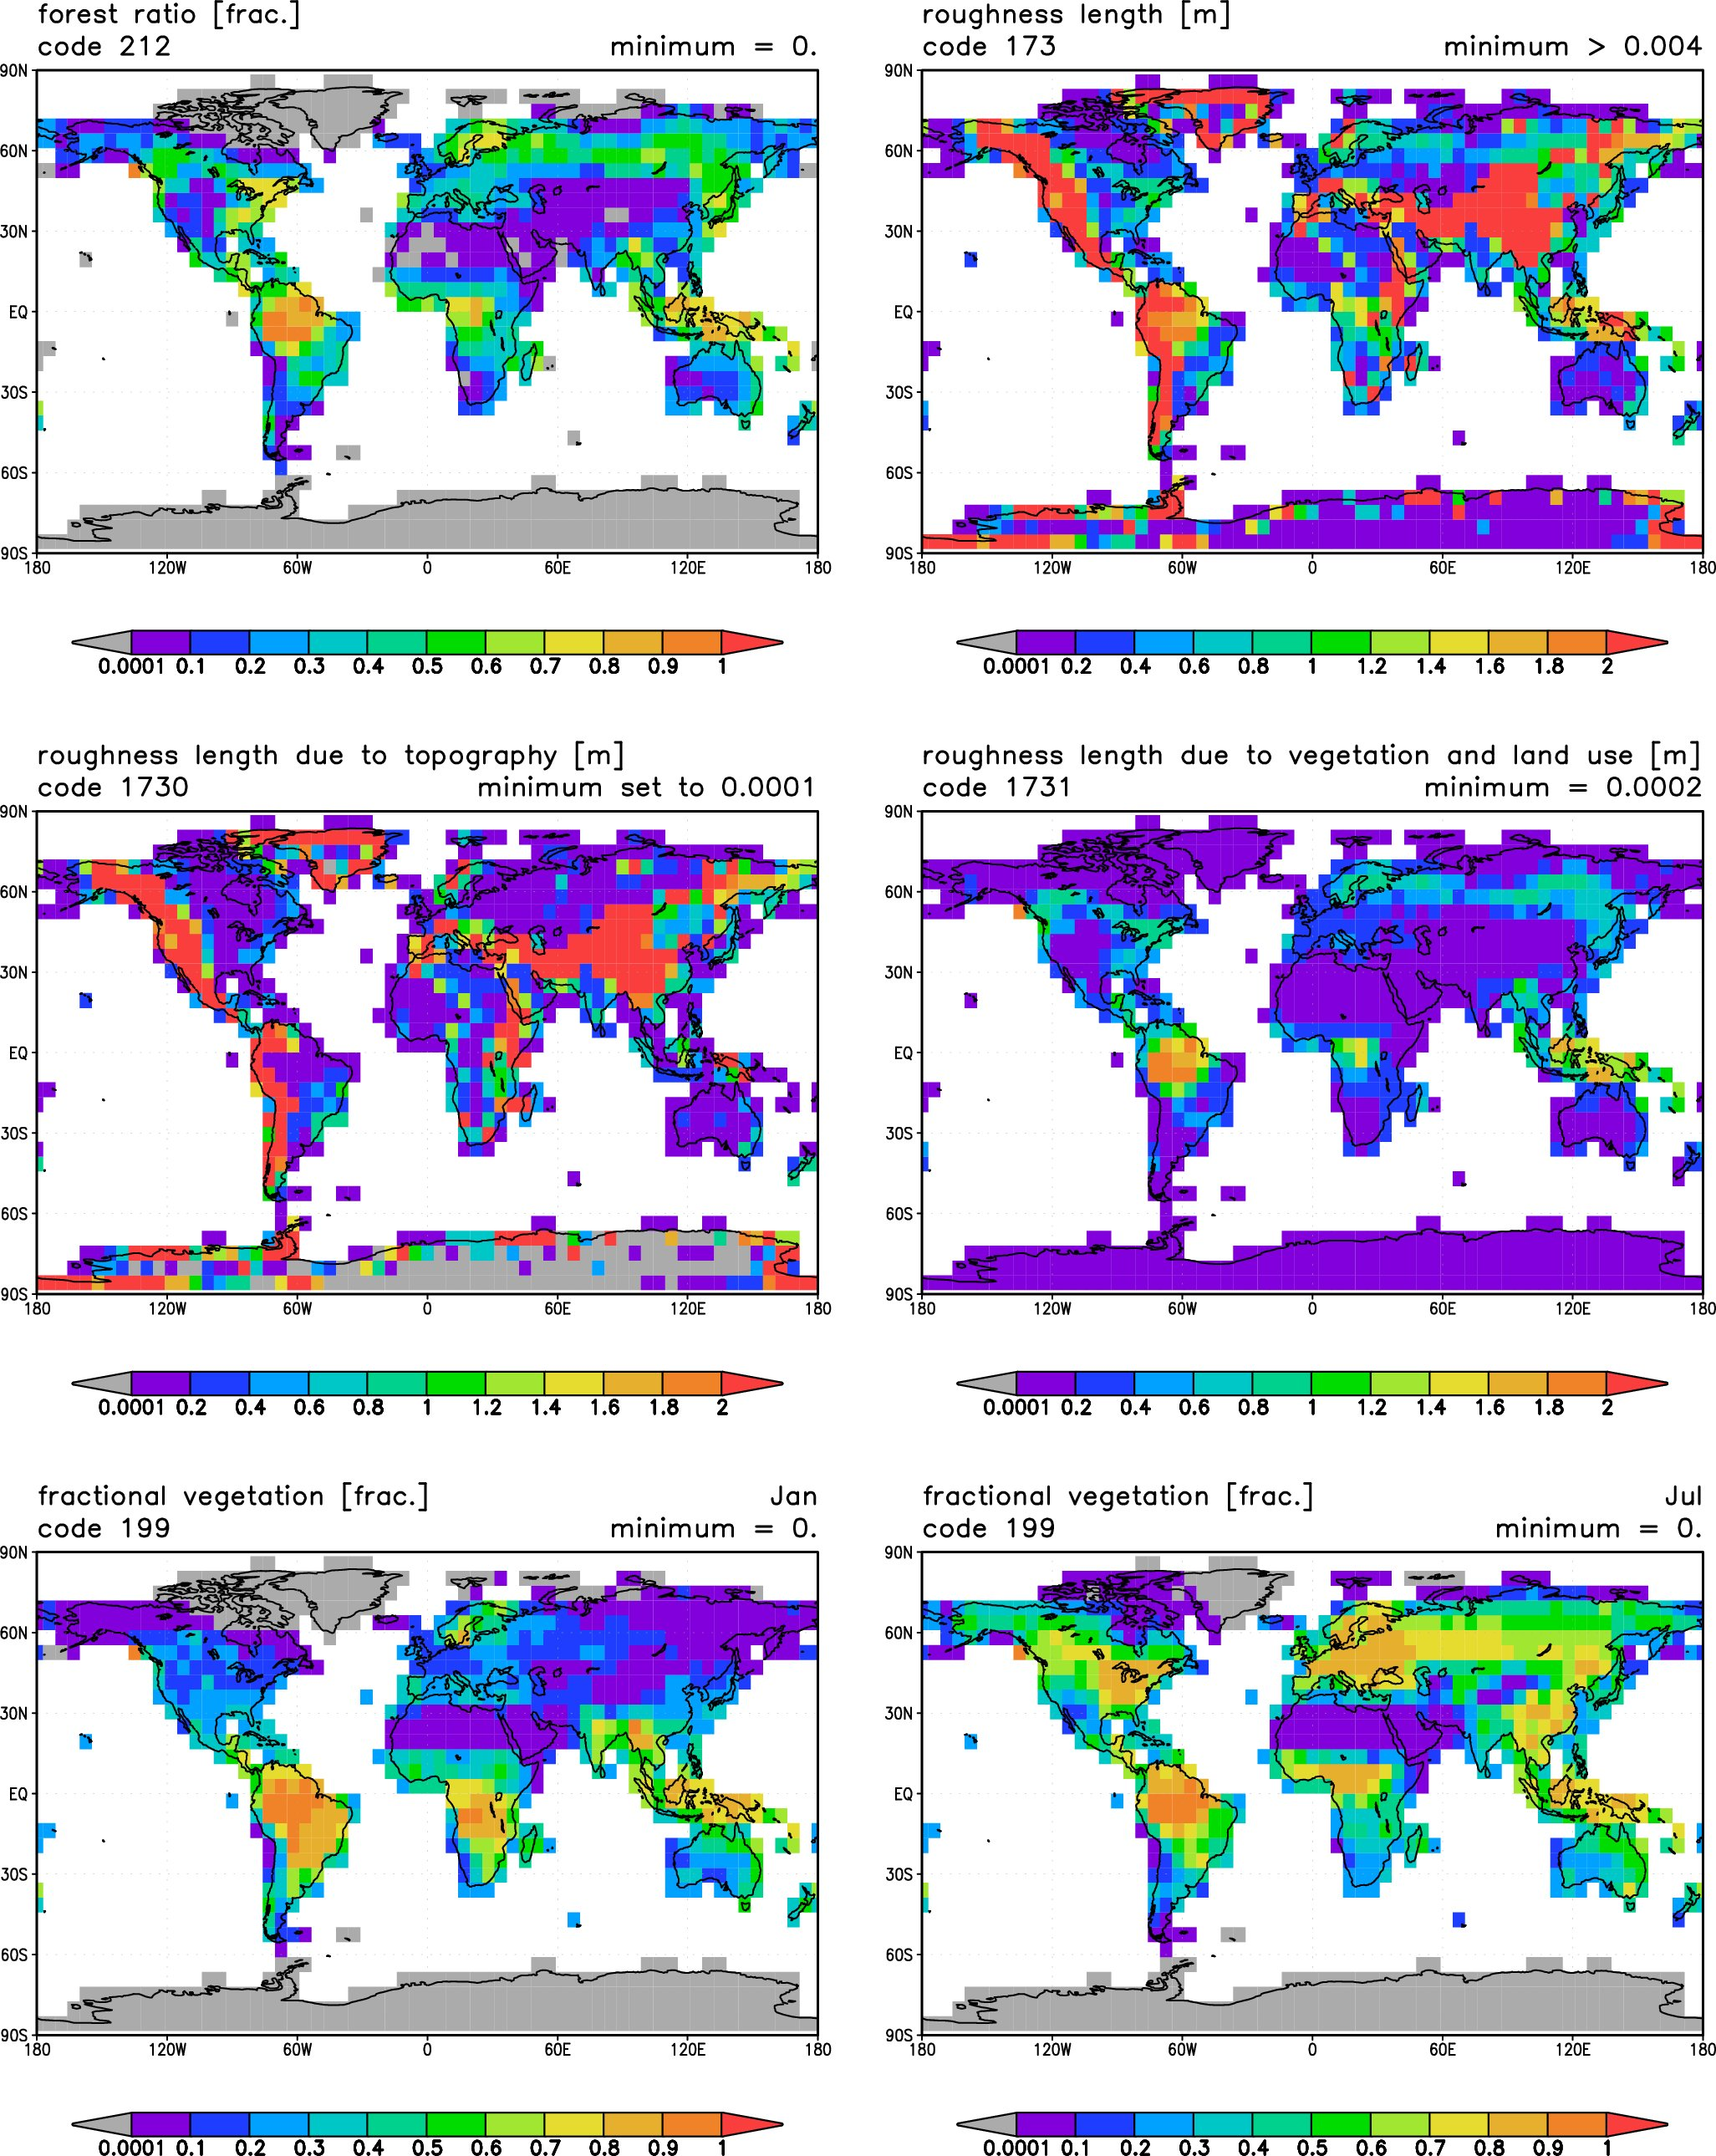
\includegraphics{silke/surface_fields_for_UG_6pic_z0}
\ec \end{figure}

\begin{figure}[ht] \bc
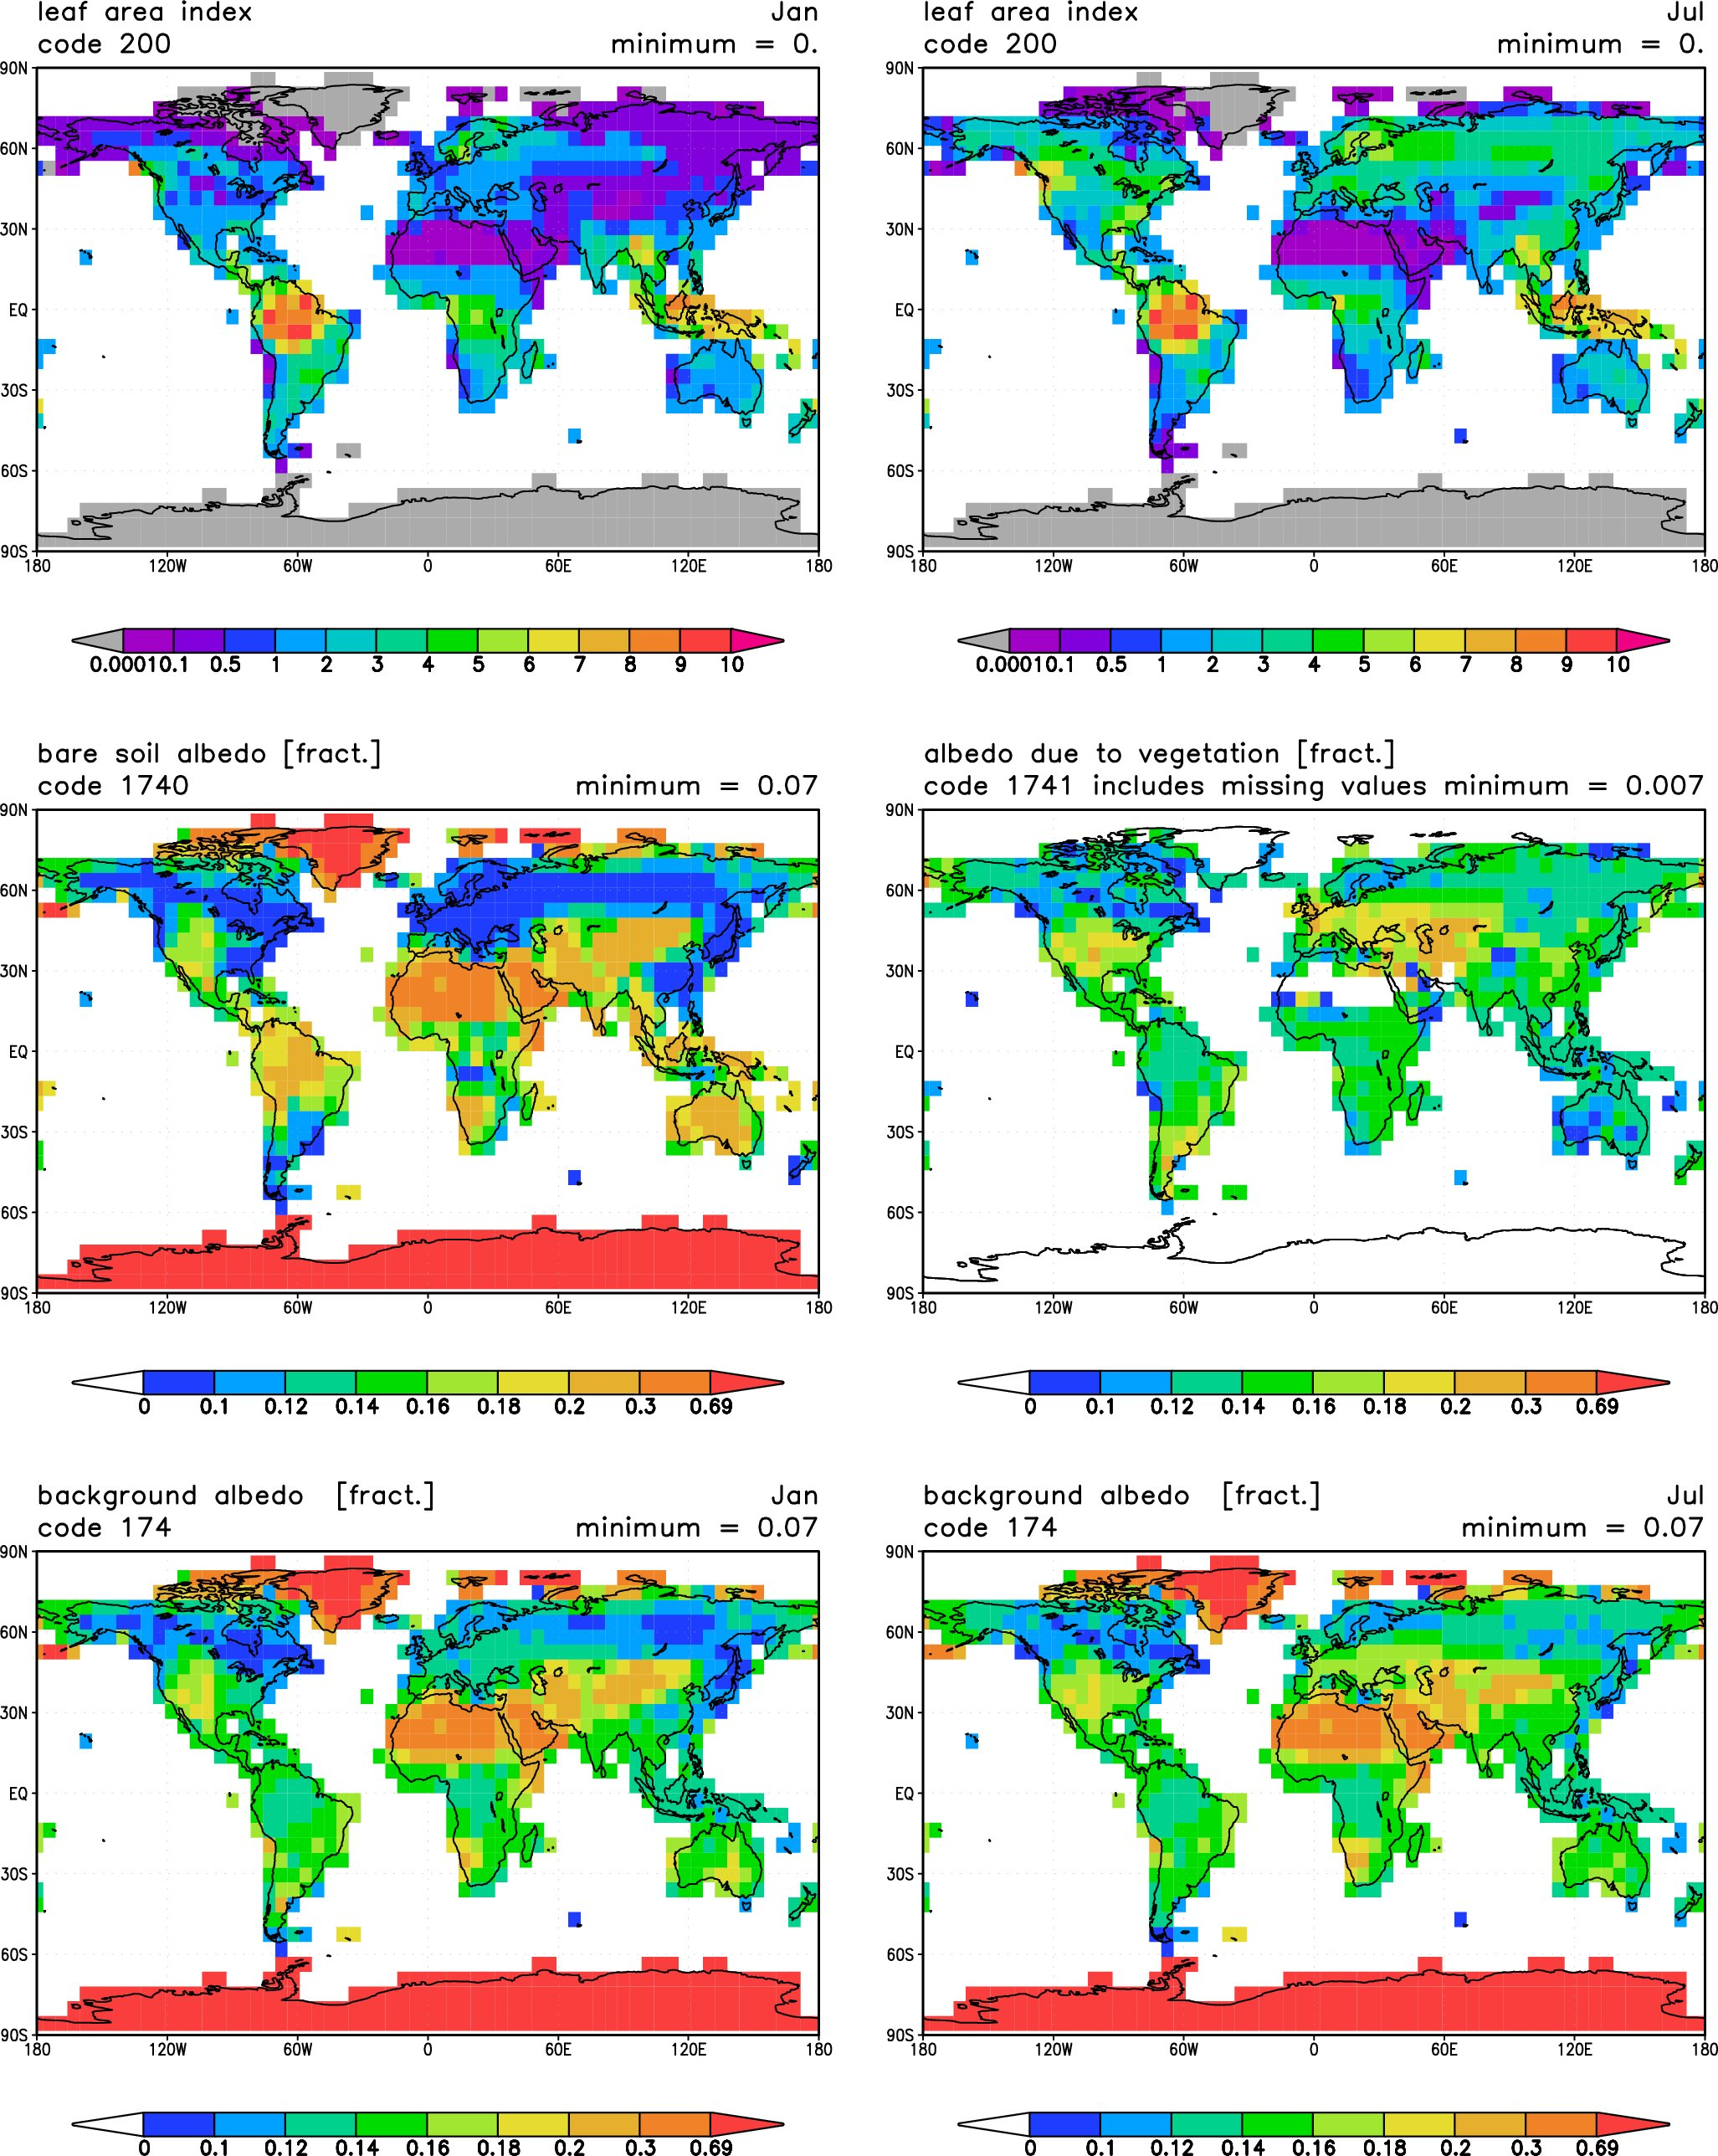
\includegraphics{silke/surface_fields_for_UG_6pic_alb}
\ec \end{figure}

% to place the following figure on top of next page instead of centered:
\clearpage
\vspace{100.ex}
% only to activate the vspace command
\begin{tabbing}
xxx \= xxx \kill
\end{tabbing}

\begin{figure}[ht] 
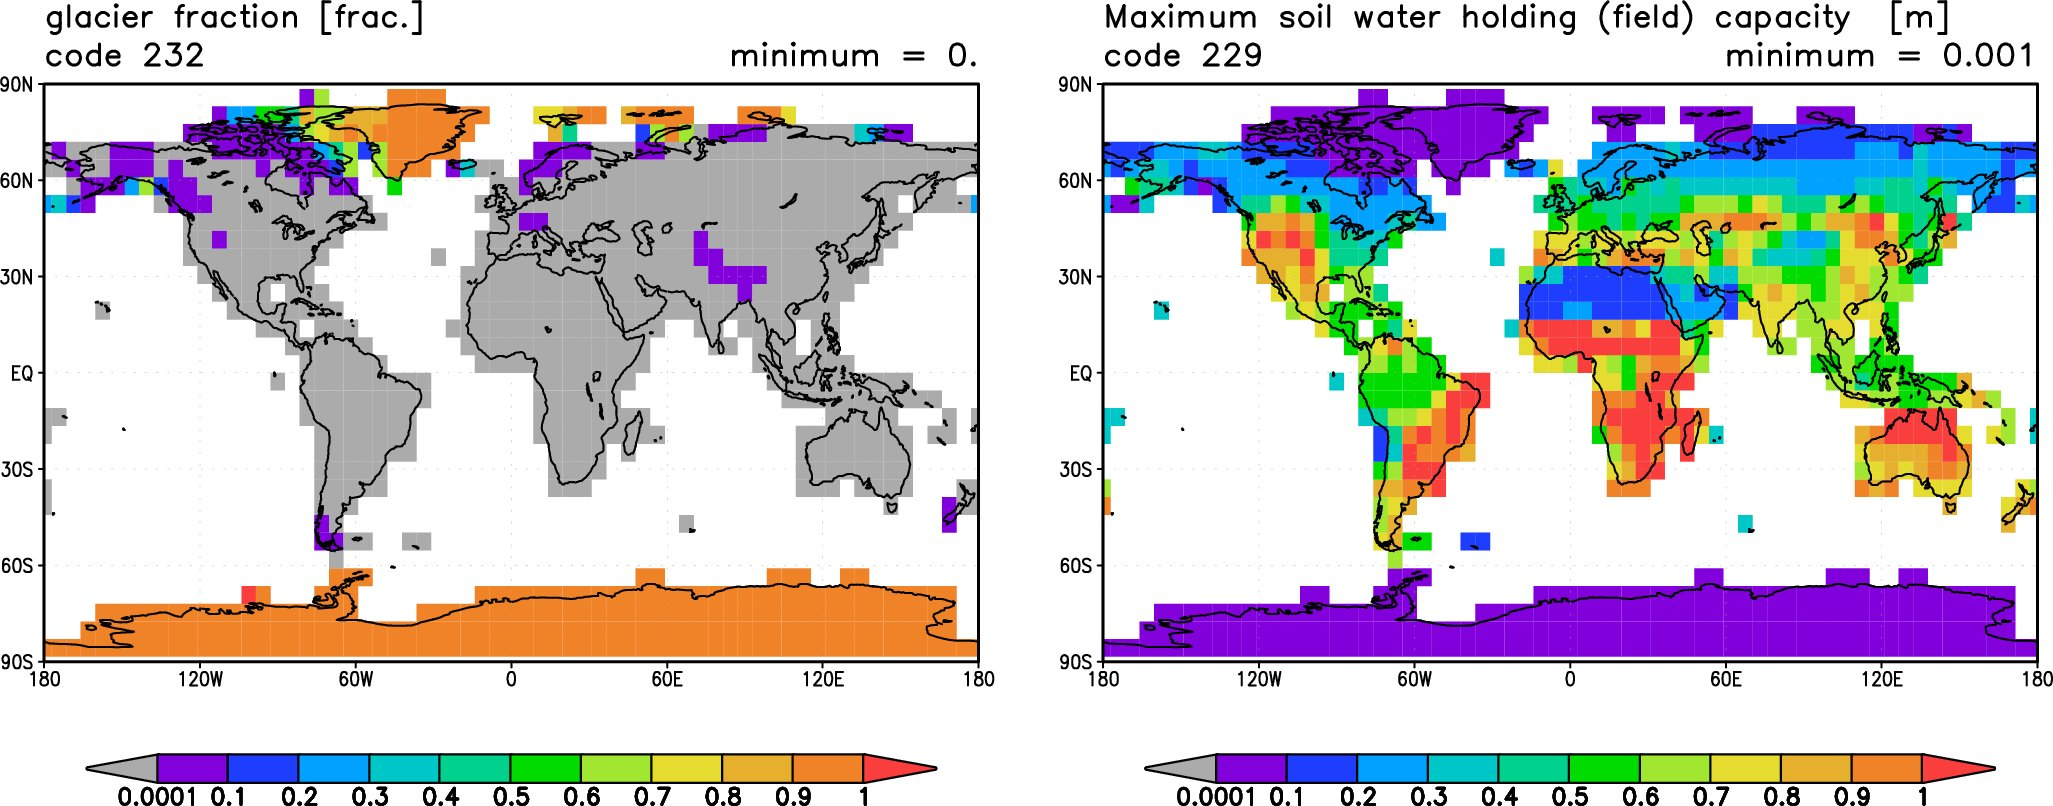
\includegraphics{silke/surface_fields_for_UG_2pic}
\end{figure}

